\documentclass{article}
\usepackage{graphicx}
\usepackage{algorithm}
\usepackage{algorithmic}
\begin{document}
\title{Specialized Cost Function for Maximizing Body Area Network Lifetime Using Global Routing Algorithms}
\author{Alvaro Prieto}
\maketitle

\begin{abstract}
TODO
\end{abstract}

\section{Introduction}
Wireless Body Area Networks (WBANs) consist of several wireless sensors located around a human body. These sensors may measure several biological signals, movement, and temperature. Due to major improvements in power consumption and constantly shrinking devices, WBANs are becoming ubiquitous. Due to the small form factor of these devices, the battery size is limited. While the sensors themselves may be extremely power efficient, all of the measured data must be transmitted over a much less efficient wireless link. One benefit of WBANs is that they rarely include more than a dozen wireless devices over a small area. This constraint allows for the use of routing techniques not suitable for larger wireless sensor networks.

There are several routing protocols designed specifically for WBANs. Braem et al. developed the CICADA protocol, which consists of a spanning tree architecture with a time-division scheme for transmission scheduling~\cite{protocol:CICADA}. The primary downside to this method is that nodes closer to the root will deplete their energy source faster due to the need to relay messages from children nodes. Other protocols focus on the reliability of the network~\cite{routing:storeandforward}. Dynamic networks are a problem with WBANs. If sensors are placed in the extremities, the network will change as the body changes positions. Quwaider et al. developed a protocol tolerant to network changes~\cite{routing:storeandforward}. They propose a store-and-forward method that maximizes the likelihood of a packet reaching its destination. Each packet is stored by multiple devices and retransmitted, which consumes more power. One solution for this problem was proposed by Ehyaie et al.~\cite{relay:networklife}, it consists of using dedicated, non-sensing, relay nodes with larger power sources. While this method increases the network lifetime, it requires more hardware. Finally, Nabi et al. propose a similar store-and-forward method, but integrates Transmit Power Adaptation (TPA)~\cite{relay:transmitpoweradaptation}. Nodes keep track of neighbors and use power control to use the smallest transmit power while maintaining a specific link quality.

For the purpose of this paper, \textbf{network lifetime} is defined as the time it takes any single node to deplete its energy source. 

In this contribution we propose a novel routing algorithm that focuses not on single devices, but the network as a whole. Current methods focus on maximizing individual device lifetime or minimizing the energy-per-bit. While those are generally good goals, certain systems require all devices functioning to be considered operational. Keeping that in mind, the proposed system maximizes the network lifetime by normalizing power use across the network.

In order to provide accurate channel conditions, RSSI measurements of an eight ED network were used as input to our simulations(\ref{sec:simulation}). Real-time hardware implementations were also run to demonstrate the algorithm(\ref{sec:hardware}). The new cost function succeeded in improving network lifetimes when run in a dynamic environment. Static environments did not produce successful results.

\begin{figure}[!htb]
\begin{center}
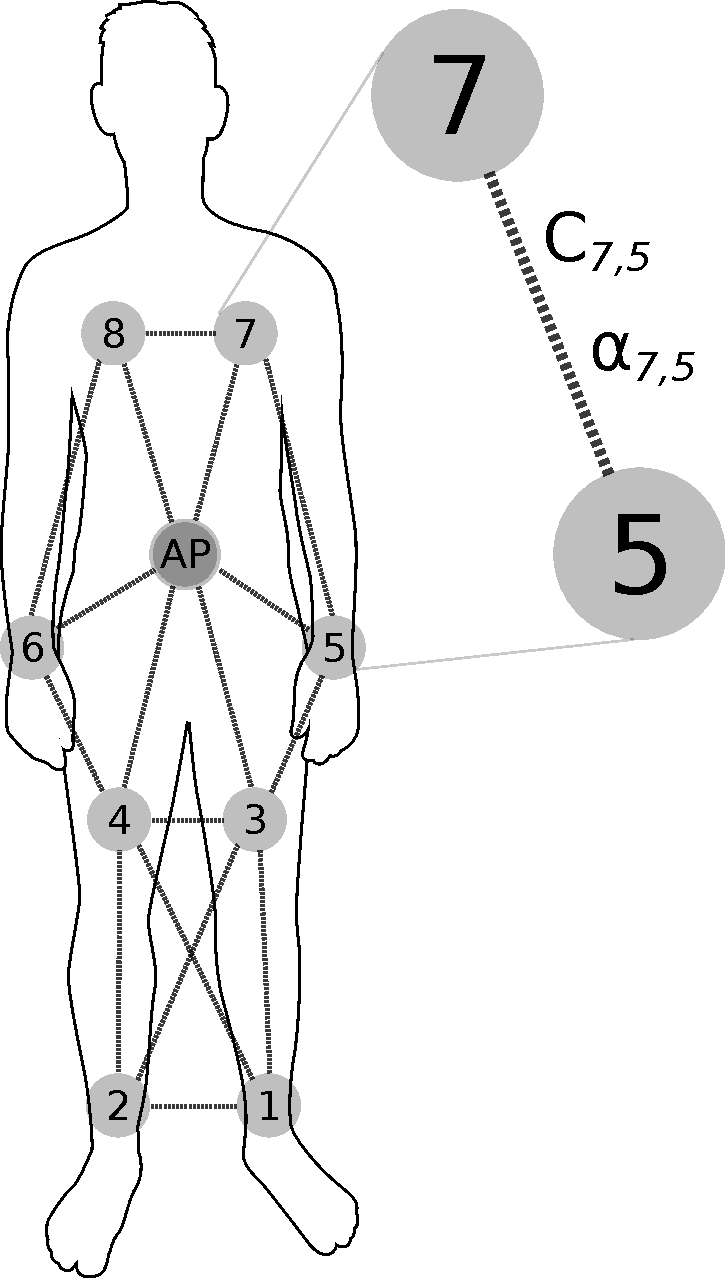
\includegraphics[width=0.5\textwidth]{figures/body.pdf}
\end{center}
\caption{Experimental Setup (Not all links shown)}
\label{fig:body}
\end{figure}

\section{Proposed Cost Function}
In the proposed system, we define a new link cost function that is then used in a routing algorithm. Traditionally, the power required to make a link possible is used as the link cost. In this case, the total energy used by a device is factored into the equation. If a device has used more energy than the others, its use as a relay will be discouraged.

\subsection{Device Energy}
Each device's normalized energy use is calculated as shown in Equation~\ref{eqn:accumulated_energy}, where $j$ denotes the device ID, $i$ is the current polling round, $\alpha_{j,k}$ is the channel attenuation for the selected link, and $RSSI^T$ is the target RSSI. The current energy used is incremented by the energy used to transmit a single packet while maintaining $RSSI^T$. The channel attenuation for the selected link,$\alpha_{j,k}$, can be seen in Equation~\ref{eqn:alpha}, where RSSI is the received power measured by device $k$ and $P_{tx}$ is the transmitted power used by device $j$. 

\subsection{Link Cost}
The actual link cost is computed by calculating the energy used by the device, \emph{if} that link is selected, and multiplying by a cost factor(Equation~\ref{eqn:link_cost}). The cost factor calculation takes the energy used by the destination device, $E^k_i$, and divides it by the current energy minimum, $E^{min}_{i}$, which is the energy used by the device with the minimum energy used by round $i$. This ratio is then raised to the power $M$, which determines how strong the effect will be. If a device's energy is much greater than the current minimum, it will be avoided as a relay.
The $M$ factor in Equation~\ref{eqn:link_cost} can be any number in $0 < M < \infty$. The cost factor is normalized so when $M=0$, it returns to the traditional cost of required power to meet the link.

Since the link costs are directly related to the destination device, they are calculated during the routing algorithm computation. For this paper, Dijkstra's algorithm~\cite{dijkstra:algorithm} is used to select the best route.

\begin{equation}
\label{eqn:alpha}
\alpha_{j,k} = \frac{RSSI}{P_{tx}}
\end{equation}
\begin{equation}
\label{eqn:accumulated_energy}
E^j_{(i)} = E^j_{(i-1)} + \frac{RSSI^T}{\alpha}
\end{equation}
\begin{equation}
\label{eqn:link_cost}
C^j_{j,k} = \frac{RSSI^T}{\alpha_{j,k}} \times \left( \frac{1+\left(\frac{E^k_i}{E^{min}_{i}} \right)^M}{2} \right)
\end{equation}

\subsection{Assumptions}
This algorithm works under several assumptions. The first being that this is a centralized network with one Access Point (AP) with virtually unlimited energy and computing power. The second is that each wireless sensor, or End Device(ED), can act as a relay for messages from other nodes. The Third is that the link quality, or channel attenuation, between all EDs and AP is known. Finally, all EDs begin with an equal energy used, that is, they all have the same energy stored. All routing calculations take place in the AP. Figure~\ref{fig:body} shows a sample network with EDs labeled 1 through 8, and one AP.

\section{Performance Analysis}
In what follows, we analyze the performance of the proposed cost function. The new cost function was tested in both simulated and experimental environments. In order to gauge the efficiency of the cost function, it will be compared to an identical system which uses a traditional link cost function. The traditional link cost function consists of the required power to meet a link with the desired $RSSI^T$. This can be achieved by setting a value of $M=0$ in the new link cost function.

Performance is determined by the time it takes any node's accumulated normalized energy to cross an arbitrary threshold. The threshold could be equivalent to the amount of energy stored in a device battery, but for this experiment, is purely arbitrary. 

\subsection{Algorithm Implementation}
Detailed pseudo-code for the routing algorithm can be found in Algorithm~\ref{alg:dijkstra}. Similarly, code for energy used calculation can be found in Algorithm~\ref{alg:energyused}.

\begin{algorithm}[!ht]
\caption{Dijkstra's Algorithm with new cost function}
\label{alg:dijkstra}
\begin{algorithmic}[1]
\FOR{$i = 1$ to \# of Nodes} 
	\STATE $node_i.visited \leftarrow 0$
	\STATE $node_i.distance \leftarrow \infty$
	\STATE $node_i.previous \leftarrow node_i$
\ENDFOR
\STATE $node_{AP}.distance \leftarrow 0$
\STATE $energy_{min} = min(node.energy)$
\WHILE{unvisited nodes available}
	\STATE $node_{source} \leftarrow $ node with smallest distance
	\FOR{$i = 1$ to \# of Links}
		\IF{$link_i.source = node_{source}$}
			\STATE $node_{dest} \leftarrow link_i.destination$
			\IF{$node_{dest}.visited = 0$}
				\STATE $cost \leftarrow link_i.power * (1 + node_{dest}.energy/energy_{min} )^M/2$
				\STATE $newdistance \leftarrow node_{source}.distance + cost$
				\IF{$distance < node_{dest}.distance$} 
				\STATE$node_{dest}.distance \leftarrow newdistance$
				\STATE$node_{dest}.previous \leftarrow node_{source}$
				\ENDIF
			\ENDIF
		\ENDIF
	\ENDFOR
	\STATE $node_{source}.visited \leftarrow 1$
\ENDWHILE
\end{algorithmic}
\end{algorithm}

\begin{algorithm}[!ht]
\caption{Energy Used Calculation}
\label{alg:energyused}
\begin{algorithmic}[1]
\FOR{$i = 1$ to \# of Nodes}
	\STATE $node_{ptr} = node_i$
	\IF{$node_{ptr}.previous = node_{ptr}$}
		\STATE No path to $node_i$
	\ELSE
		\WHILE{$node_{ptr}.previous \neq node_{ptr}$}
			\STATE $link_{ptr} \leftarrow $ link between $node_{ptr}$ and $node_{ptr}.previous$
			\STATE $node_{ptr}.energy += link_{ptr}.power$
			\STATE $node_{ptr} \leftarrow = node_{ptr}.previous$
		\ENDWHILE
	\ENDIF
\ENDFOR
\end{algorithmic}
\end{algorithm}


\section{Simulation}\label{sec:simulation}
In order to test the new cost function in an efficient manner, a simulation was used. Measurements of real channel data were acquired by running the procedure described in~\ref{subsec:cycleofoperations} without the routing or power control enabled. Each ED continuously sampled RSSI data from all other devices and transmitted it to the host. 

Two experimental setups were used to capture RSSI data. For the first, the subject remained relatively static in a sitting position. The second consisted of a more dynamic environment, where the subject walked around a room as seen in Figure~\ref{fig:floorplan}. 

A set of captured RSSI tables (as seen in Table~\ref{tab:rssi}) were fed into the simulation, which proceeded to run the routing algorithm. The simulation produced energy use data, along with power settings, and routes taken for all devices.

\section{Hardware Implementation}\label{sec:hardware}
In order to verify the new cost function in a real environment, a hardware platform was developed and used. The system function in a similar fashion to the simulation, except that the actual routing and power control data was fed back to the ED's.

\subsection{Hardware Platform}
The hardware platform used for this test consists of the Texas Instruments (TI) EZ430-RF2500. This device includes both an MSP430F2274 microcontroller along with a CC2500 2.4GHz transceiver. The CC2500 is configured to run at 250kbps.
A single device, labeled the Access Point (AP), is connected via a USB to Serial link, running at 115200 BAUD, to the host computer. All other devices, labeled End Devices (EDs), are battery powered. In this implementation, the AP acts only as a bridge between the host and the end devices. All routing and power control calculations are done on the host.

The host is a laptop computer with an Intel(R) Core(TM) i5-2410M CPU and 4GB of RAM. Eight EDs were placed on a 170cm, 70kg male subject as shown in Figure~\ref{fig:body}. The host was carried on a backpack and connected to the AP via a USB cable. The data was sampled, and the routing algorithm was run, at a rate of 5Hz. This sampling rate is appropriate as long as the subject, or its environment, does not move faster than this.$\ll$What was the name for this?$\gg$ If data needs to be sampled at a faster rate, some hardware and firmware changes might be necessary, but the host software will still work.

For both simulation and hardware experiments, the target RSSI ($RSSI^T$) was arbitrarily chosen to be $-60 dBm$.

\begin{figure}[!htb]
\begin{center}
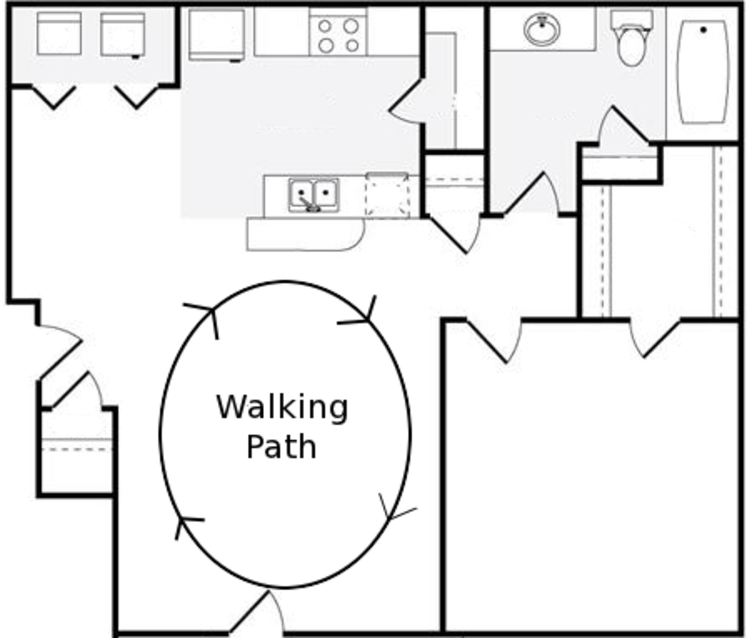
\includegraphics[width=0.6\textwidth]{figures/floorplan.pdf}
\end{center}
\caption{Walking environment.}
\label{fig:floorplan}
\end{figure}

\subsection{Cycle of Operations}\label{subsec:cycleofoperations}
A normal cycle of operations with $n$ devices works as follows:

\begin{algorithmic}[1]
\STATE AP sends synchronization beacon which includes routing and power control tables.
\STATE Each ED transmits its own RSSI table back to the AP, while simultaneously listening to other ED messages and storing the received power from each.
\STATE Once all EDs have transmitted their data, the AP sends a table with the RSSI data from all devices. (See Table~\ref{tab:rssi} for an example)
\STATE The host uses the RSSI table to compute the routes along with the required powers to meet the selected links.
\STATE The host sends both routing and power tables back to the AP so that a new cycle may begin.
\end{algorithmic}

\begin{table}[htb]
\begin{tabular}{|c|c|c|c|c|c|c|c|c|c|}
\hline  & AP & ED1 & ED2 & ED3 & ED4 & ED5 & ED6 & ED7 & ED8 \\ 
\hline AP & - & -60 & -60 & -60 & -60.5 & -60.5 & -60.5 & -60 & -79.5 \\ 
\hline ED1 & -66 & - & -62 & -75 & -63.5 & -69 & -75.5 & -73 & -67.5 \\ 
\hline ED2 & -72 & -61.5 & - & -80 & -69 & -70 & -74 & -75 & -66 \\ 
\hline ED3 & -77.5 & -74.5 & -80.5 & - & -67.5 & -70 & -72.5 & -70.5 & -70 \\ 
\hline ED4 & -39 & -63 & -69.5 & -67 & - & -82.5 & -74.5 & -69 & -65.5 \\ 
\hline ED5 & -67.5 & -68 & -71 & -69.5 & -84 & - & -55.5 & -51.5 & -62 \\ 
\hline ED6 & -67 & -75 & -75 & -72.5 & -75 & -55.5 & - & -44.5 & -53 \\ 
\hline ED7 & -46 & -70 & -77.5 & -70.5 & -69 & -50.5 & -45 & - & -51.5 \\ 
\hline ED8 & -78 & -67.5 & -66.5 & -71 & -66 & -62 & -54 & -51.5 & - \\ 
\hline 
\end{tabular} 
\caption{Sample RSSI Table}
\label{tab:rssi}
\end{table}


\subsection{Details}
To minimize the number of control packets from being transmitted, the EDs are not individually polled. The only control packet that is sent is the synchronization beacon, which also carries the routing and power tables. Once the EDs are synchronized, they transmit their data on a pre-defined schedule to avoid collisions. Each ED has a network ID ranging from 1 to $n$. The time between synchronization packets is divided into time-slots than are used by each ED. The time slot used depends on the network ID of each device. This removes the need to come up with time schedules during runtime.

The routing table is a simple array which lists the destination for each ED packet. The ED does not need to know the entire route its packets will take, but only next device in the path. Similarly, the power table lists the transmit power setting each device needs to use. The size of these tables is directly proportional to the number of devices in the network.

\section{Results}

Due to the similarities between the simulation and hardware implementation (they both use real RSSI data), the results were fairly similar. If fed with the same RSSI data, the algorithm will always produce the same results. The only difference with the hardware implementation is that the RSSI table is reduced due to power control. Since each ED only uses enough transmit power to reach a specific ED, others might not get the message. This was not a problem when the hardware experiment was run.

\begin{figure}[!ht]
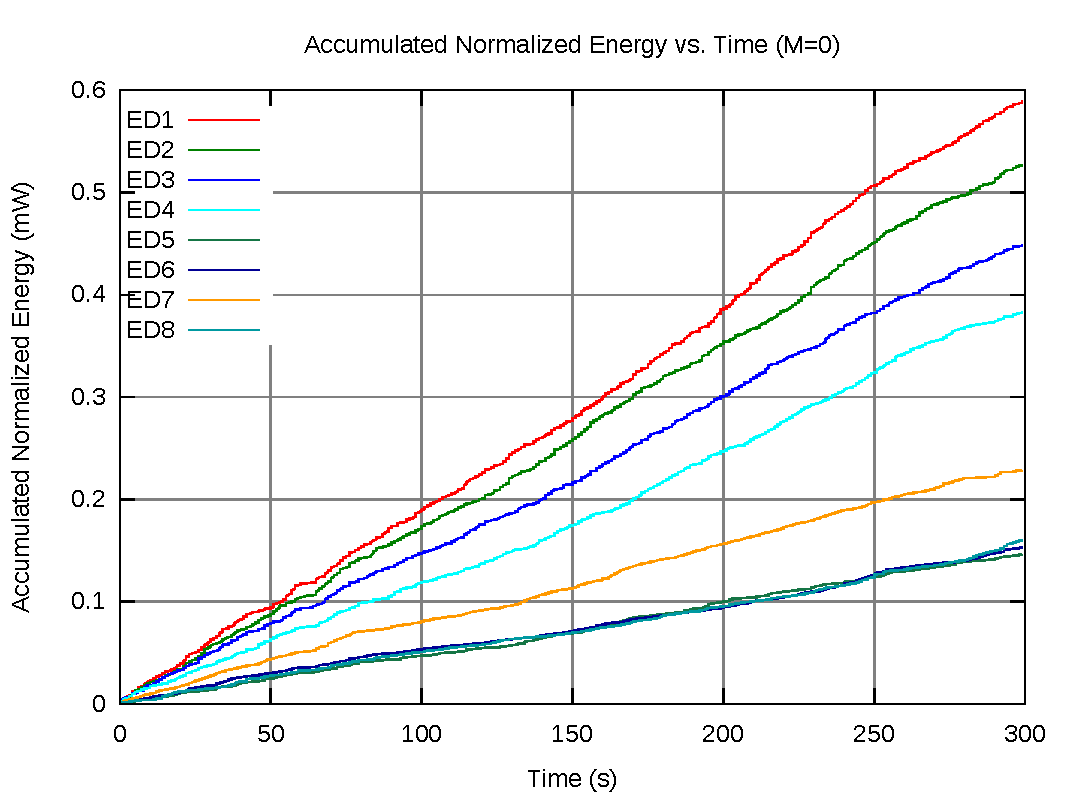
\includegraphics[width=0.8\textwidth]{figures/sit1-c0.pdf}
\caption{Sitting M=0}
\label{fig:sit1-c0}
\end{figure}

\begin{figure}[!ht]
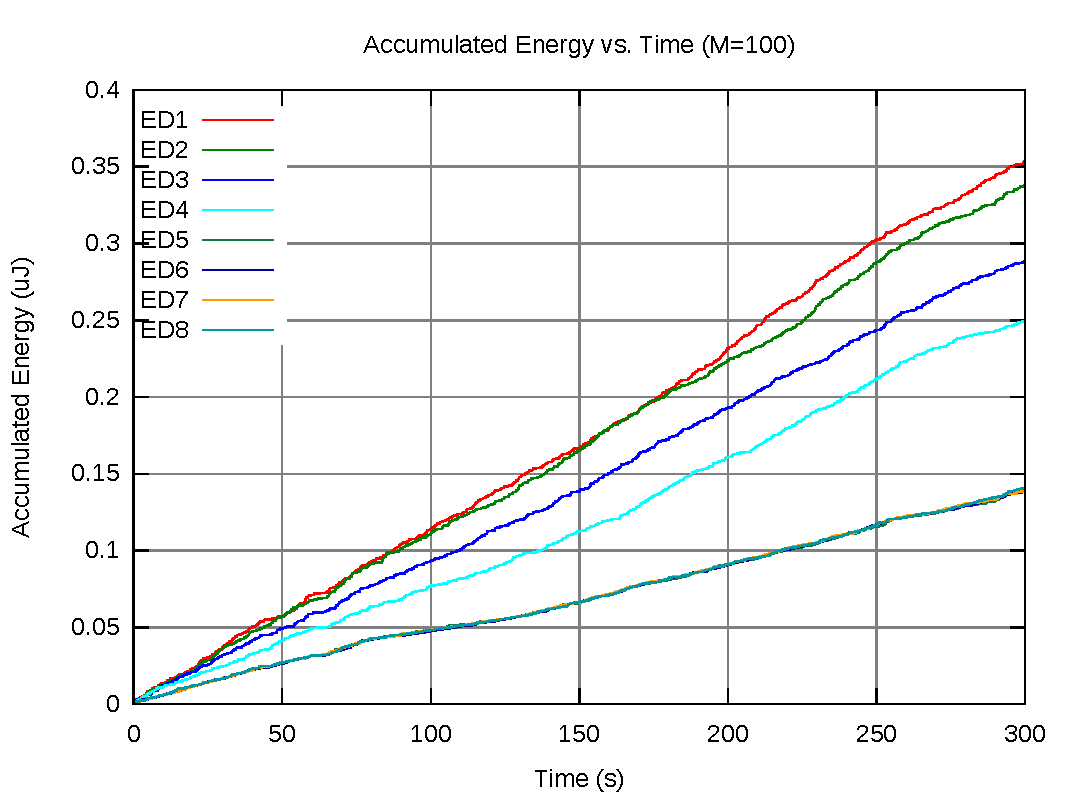
\includegraphics[width=0.8\textwidth]{figures/sit1-c100.pdf}
\caption{Sitting M=100}
\label{fig:sit1-c100}
\end{figure}

Figures~\ref{fig:sit1-c0}~and~\ref{fig:sit1-c100} show the resulting accumulated energies while the subject was in a sitting position. The experiment was run with both an $M=0$ as a reference, and $M=100$. Unfortunately, the results with a static subject were rather neutral. All EDs consume energy at different rates for both $M=0$ and $M=100$.

Figures~\ref{fig:walk2-c0}~and~\ref{fig:walk2-c100}, on the other hand, show an increase in network lifetime. At the end of the 5 minute sampling time with $M=0$, the device which consumed the most power was ED7 with approximately 1.7 mW. On the other hand, with $M=100$, all EDs consume power in a uniform fashion and end up with less than 1.3 mW each. One important observation is that the network with $M=0$ consumed less overall power (~9.6mW) than the one with $M=100$ (~10.1mW). This is expected, due to the fact that the new cost function specifically avoids the most efficient path for a specific node in favor of the most efficient path for the whole network. While more energy is consumed overall, no single ED consumes significantly more power. 

To demonstrate the network lifetime improvement, an ED will be considered have depleted it's power source after consuming 1mW of normalized energy. In the previous example, the trial with $M=0$ reaches 1mW after approximately 175 seconds, while the case with $M=100$ reaches it around 240 seconds.

\begin{figure}[!ht]
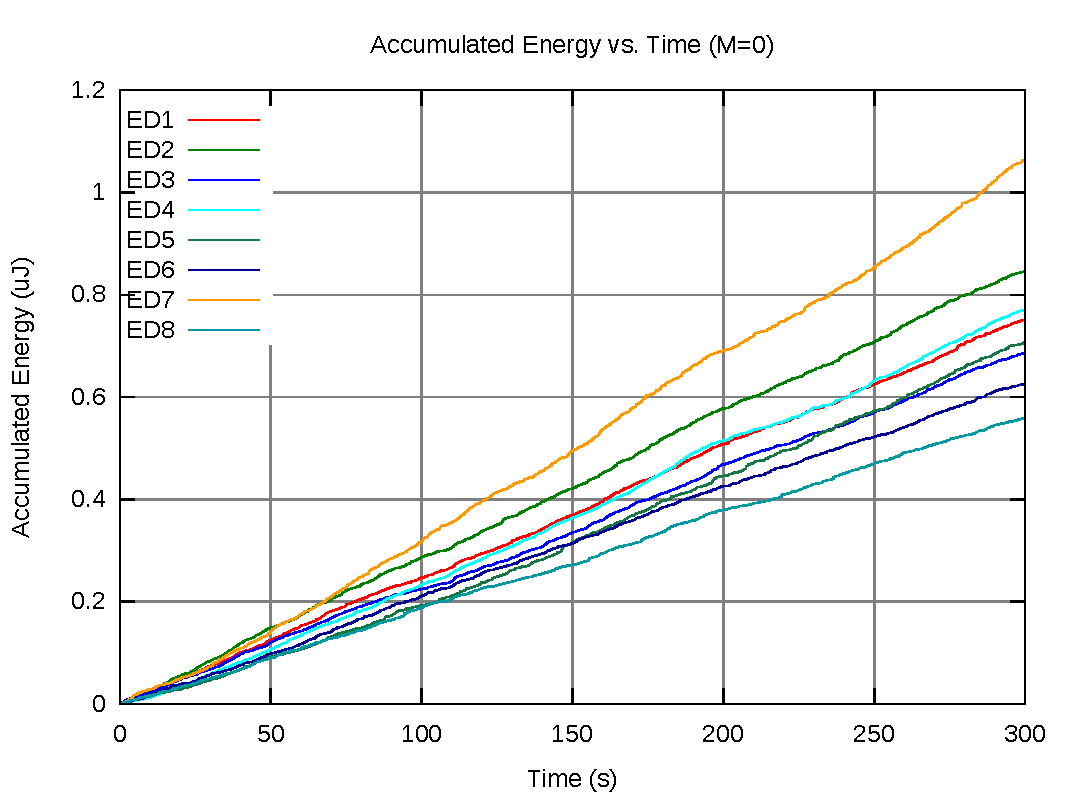
\includegraphics[width=0.8\textwidth]{figures/walk2-c0.pdf}
\caption{Walking M=0}
\label{fig:walk2-c0}
\end{figure}

\begin{figure}[!ht]
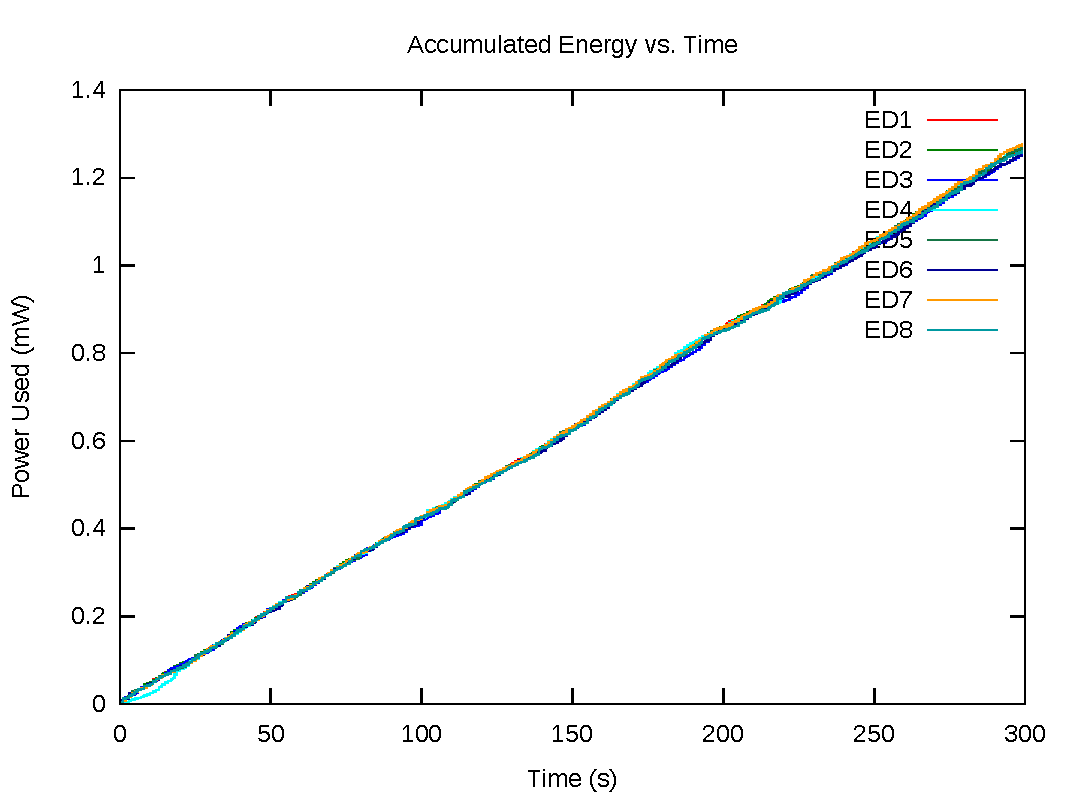
\includegraphics[width=0.8\textwidth]{figures/walk2-c100.pdf}
\caption{Walking M=100}
\label{fig:walk2-c100}
\end{figure}

A good example of the algorithm working was a result of hardware problems. During of the experiments, a single ED went off-line for several seconds and was manually restarted. Figure~\ref{fig:walk4-c100} shows the effect the ED failure had on the network. Because a device that is powered off does not consume power, it became the one with the least energy used. When it returned to the network, it was immediately used as a relay by other nodes. 

\begin{figure}[!ht]
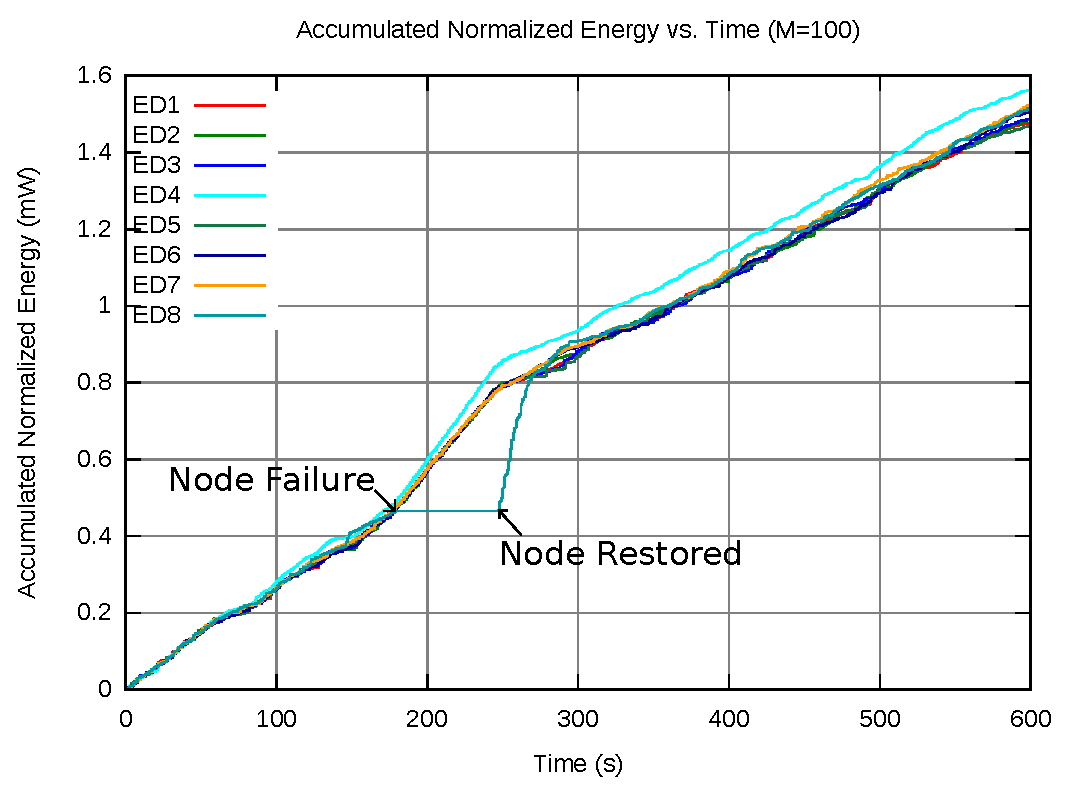
\includegraphics[width=0.8\textwidth]{figures/walk4-c100.pdf}
\caption{Walking M=100}
\label{fig:walk4-c100}
\end{figure}

\section{Conclusion}
After analyzing the results, the new link cost function successfully improves network lifetime. The new cost function outperformed the traditional one in trials dealing with a dynamic environment, where the subject was walking. When the subject was not moving, both link costs performed about the same. Note that, in this case, performance is with respect to network lifetime, and not overall power consumption.
While the new link cost was successful, there is room for improvement. One improvement that can be done deals with the example from Figure~\ref{fig:walk4-c100}. While the failed ED was not part of the network, it was still taken into account when it came to link cost calculation. A better implementation would not include off-line devices in the calculation. A second modification would relate actual battery, or other power source, charge to the algorithm. This would allow for devices to join and leave the network while maintaining proper operation. It would also allow devices with different power sources to be included and used.

\bibliography{sources/thesis.bib}{}
\bibliographystyle{plain}

\end{document}